\documentclass[11pt, a4paper]{article}

\usepackage{ctex}
\usepackage{geometry}
\usepackage{amsmath}
\usepackage{amssymb}

\geometry{bottom=2cm, top=2cm, left=1.5cm, right=1.5cm}
\setlength{\arraycolsep}{5pt}
\renewcommand{\arraystretch}{2.5}

\begin{document}
	
\title{微分方程实验二:二次有限元方法求解两点边值问题}
\author{15336134 莫凡}
\maketitle
	
\section{实验假设}

这次实验是实验一:使用线性有限元求解两点边值问题的改进。使用二次有限元方法求解两点边值问题
\begin{equation}
	\begin{array}{c}
	Lu=-\dfrac{\mathrm{d}}{\mathrm{d}x}\left(p\dfrac{\mathrm{d}u}{\mathrm{d}x}\right)+qu=f\quad x\in (a, b)\\
	u(a)=0,u'(b)=0
	\end{array}
\end{equation}
	
仍然假设具体问题为书后P47中的
\begin{equation}
	p=1,~q=\dfrac{\pi^2}{4},~f=\dfrac{\pi^2}{2}\sin\dfrac{\pi}{2}x,~a=0,~b=0
\end{equation}

(只是为了测试方便,程序可以在任意问题上运行)

\section{理论分析与实验过程}

通过Galerkin方法推导出二次函数插值的方程组。首先通过拉格朗日插值得到函数$\varphi_i(x)$和$\varphi_{i.5}(x)$,有
\begin{equation}
	\varphi_i(x)=\left\{
	\begin{array}{cr}
		\left(2\dfrac{x_i-x}{h_i}-1\right)\left(\dfrac{x_i-x}{h_i}-1\right) & x_{i-1}\le x<x_i\\
		\left(2\dfrac{x-x_i}{h_{i+1}}-1\right)\left(\dfrac{x-x_i}{h_{i+1}}-1\right) & x_{i}\le x\le x_{i+1}\\
		0 & \text{otherwise}
	\end{array}
	\right.
\end{equation}

\begin{equation}
	\varphi_{i.5}(x)=\left\{
	\begin{array}{cr}
		4\dfrac{x-x_i}{h_{i+1}}\left(1-\dfrac{x-x_i}{h_{i+1}}\right) & x_{i}\le x\le x_{i+1}\\
		0 & \text{otherwise}
	\end{array}
	\right.
\end{equation}

接下来对他们求导数

\begin{equation}
	\varphi_i'(x)=\left\{
	\begin{array}{cr}
		\dfrac{3h_i+4x-4x_i}{h_i^2} & x_{i-1}\le x<x_i\\
		\dfrac{-3h_{i+1}+4x-4x_i}{h_{i+1}^2} & x_{i}\le x\le x_{i+1}\\
		0 & \text{otherwise}
	\end{array}
	\right.
\end{equation}

\begin{equation}
	\varphi_{i.5}'(x)=\left\{
	\begin{array}{cr}
		\dfrac{-3h_{i+1}+4x-4x_i}{h_{i+1}^2} & x_{i}\le x\le x_{i+1}\\
		0 & \text{otherwise}
	\end{array}
	\right.
\end{equation}

通过Galerkin方程可以发现,刚度矩阵是若干个$3\times 3$的对称矩阵摆在对角线上相加。每个元素可以表示成双线性积分。公式实在是太长了就不打上来了。

最后得到刚度矩阵,由于它显然是一个严格对角占优的大型稀疏矩阵,所以最后使用Jacobi方法求出方程的解。具体流程请参见代码及其中简明注释。

\section{实验结果}
得到了一个效果不是很好的结果,应该是哪里出了一点问题,本着实事求是的原则就这么贴上来,日后再回来仔细修正

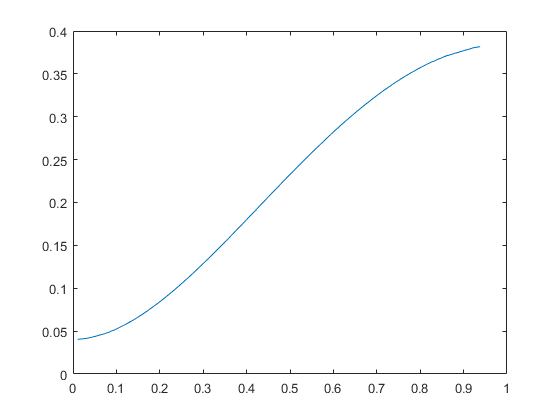
\includegraphics[width=200pt]{res.png}

在一些很简单的多项式函数上没有问题。

\section{实验心得}

要时刻注意数组下标加一减一的问题。MATLAB的函数句柄在判断返回值类型的时候会出现一些问题。要善于利用多种多样的计算工具。讨论有助于交流经验及发现问题。


\section{附件}
\begin{itemize}
	\item script.m 运行主脚本
	\item solve.m 二次元方法程序
	\item phi\_i.m $\varphi_i$函数的实现
	\item phi\_i\_5.m $\varphi_{i.5}$函数的实现
	\item dphi\_i.m $\varphi_i$函数的导数
	\item dphi\_i\_5.m $\varphi_{i.5}$函数的导数
	\item plotans.m 用于展现最终插值结果
\end{itemize}
\end{document}